\documentclass[12pt,a4paper]{article}
\usepackage[utf8]{vietnam}
\usepackage{amsmath,amssymb}
\usepackage{geometry}
\geometry{top=1.5cm,bottom=1.2cm,left=1.4cm,right=1.4cm,headheight=28pt,headsep=12pt,footskip=18pt}
\usepackage{tikz}
\usepackage{xcolor}
\usepackage{enumerate}
\usepackage{graphicx}
\usepackage[version=4]{mhchem}
\usepackage{fancyhdr}
\usepackage{ex_test}

\renewcommand{\baselinestretch}{0.96}
\setlength{\parskip}{0pt}

\definecolor{hfRed}{RGB}{211,47,47}
\definecolor{hfGreen}{RGB}{139,195,144}

\pagestyle{fancy}
\fancyhf{}
\fancyhead[L]{\small\itshape\color{hfRed} Tài liệu lưu hành nội bộ}
\fancyhead[R]{\small\itshape\color{hfRed} Thầy \textbf{TRẦN VĂN THẠNH} - 0777.470.803}
\renewcommand{\headrulewidth}{0.8pt}
\renewcommand{\headrule}{\hbox to\headwidth{\color{hfGreen}\leaders\hrule height \headrulewidth\hfill}}

\fancyfoot[L]{\small\itshape\color{hfRed} CS1: 6/15 Nguyễn Hoàng, P. Kim Long, TP Huế \quad|\quad CS2: 24 Đặng Thái Thân, TP Huế}
\fancyfoot[R]{\small\bfseries\color{hfRed} Trang \thepage}
\renewcommand{\footrulewidth}{0.8pt}
\renewcommand{\footrule}{\hbox to\headwidth{\color{hfGreen}\leaders\hrule height \footrulewidth\hfill}}

\fancypagestyle{firstpage}{
  \fancyhf{}
  \renewcommand{\headrulewidth}{0pt}
  \fancyfoot[L]{\small\itshape\color{hfRed} CS1: 6/15 Nguyễn Hoàng, P. Kim Long, TP Huế \quad|\quad CS2: 24 Đặng Thái Thân, TP Huế}
  \fancyfoot[R]{\small\bfseries\color{hfRed} Trang \thepage}
  \renewcommand{\footrulewidth}{0.8pt}
  \renewcommand{\footrule}{\hbox to\headwidth{\color{hfGreen}\leaders\hrule height \footrulewidth\hfill}}
}

\begin{document}
\thispagestyle{firstpage}

\noindent
\begin{minipage}[t]{0.44\textwidth}
	\centering\fontsize{10pt}{12pt}\selectfont
	\textbf{SỞ GIÁO DỤC VÀ ĐÀO TẠO THỪA THIÊN HUẾ}\\
	\textbf{ĐỀ CHÍNH THỨC}\\
	\textit{(Đề thi có 04 trang)}
\end{minipage}\hfill
\begin{minipage}[t]{0.54\textwidth}
	\centering\small
	\textbf{ĐỀ KIỂM TRA ĐỊNH KỲ CHƯƠNG 1 (CÂN BẰNG HÓA HỌC)}\\
	\textbf{MÔN: HOÁ HỌC -- LỚP 11}\\
	\textit{Thời gian làm bài: 45 phút (không kể thời gian phát đề)}\\
	\fbox{\textbf{MÃ ĐỀ: 102}}
\end{minipage}

\smallskip
\noindent\hrulefill
\smallskip

\noindent\textbf{Họ, tên thí sinh:} \dotfill\ \textbf{Lớp:} \dotfill\ \textbf{Số báo danh:} \dotfill

\smallskip
\noindent\textit{(Cho biết nguyên tử khối: H = 1; C = 12; N = 14; O = 16; Na = 23; Al = 27; S = 32; Cl = 35,5; K = 39; Ca = 40; Fe = 56; Cu = 64; Ba = 137).}
\smallskip

\noindent
\textbf{PHẦN I (4,5 điểm -- 18 câu): Câu trắc nghiệm nhiều phương án lựa chọn.}\\
\textit{Thí sinh trả lời từ câu 1 đến câu 18. Mỗi câu hỏi thí sinh chỉ chọn một phương án.}

\Opensolutionfile{ans}[ans-hoa11-de02hs]

\begin{ex}
Cân bằng hóa học liên quan đến loại phản ứng
\choice
{Không thuận nghịch.}
{Thuận nghịch.}
{Một chiều.}
{Oxi hóa – khử.}
\loigiai{}
\end{ex}

\begin{ex}
Yếu tố nào sau đây luôn luôn không làm dịch chuyển cân bằng của hệ phản ứng?
\choice
{Nhiệt độ.}
{Áp suất.}
{Nồng độ.}
{Chất xúc tác.}
\loigiai{}
\end{ex}

\begin{ex}
Khi phản ứng thuận nghịch ở trạng thái cân bằng thì nó
\choice
{Không xảy ra nữa.}
{Vẫn tiếp tục xảy ra.}
{Chỉ xảy ra theo chiều thuận.}
{Chỉ xảy ra theo chiều nghịch.}
\loigiai{}
\end{ex}

\begin{ex}
\textbf{[CTST - SGK]} Yếu tố nào sau đây luôn luôn không làm dịch chuyển cân bằng của hệ phản ứng?
\choice
{Nhiệt độ}
{Áp suất}
{Nồng độ}
{Chất xúc tác}
\loigiai{}
\end{ex}

\begin{ex}
Chất nào sau là acid theo thuyết Brønsted -- Lowry?
\choice
{$\ce{NaNO3}$}
{$\ce{HBrO3}$}
{$\ce{K2SO4}$}
{$\ce{CsOH}$}
\loigiai{}
\end{ex}

\begin{ex}
Phản ứng nào dưới đây không phải là phản ứng acid-base?
\choice
{$\ce{HCl + KOH -> KCl + H2O}$}
{$\ce{H2SO4 + CaO -> CaSO4 + H2O}$}
{$\ce{H2SO4 + BaCl2 -> BaSO4 v + 2HCl}$}
{$\ce{2HNO3 + Cu(OH)2 -> Cu(NO3)2 + 2H2O}$}
\loigiai{}
\end{ex}

\begin{ex}
Các dung dịch sau đây có cùng nồng độ $0{,}10\text{ mol/L}$, dung dịch nào dẫn điện kém nhất?
\choice
{$\ce{HCl}$}
{$\ce{HF}$}
{$\ce{HI}$}
{$\ce{HBr}$}
\loigiai{}
\end{ex}

\begin{ex}
Hòa tan một acid vào nước ở $25^\circ\text{C}$, kết quả là:
\choice
{$[\ce{H+}] < [\ce{OH-}]$}
{$[\ce{H+}] = [\ce{OH-}]$}
{$[\ce{H+}] > [\ce{OH-}]$}
{$[\ce{H+}][\ce{OH-}] > 1{,}0 \cdot 10^{-14}$}
\loigiai{}
\end{ex}

\begin{ex}
Chất nào sau đây không dẫn điện được?
\choice
{$\ce{KCl}$ rắn, khan}
{$\ce{CaCl2}$ nóng chảy}
{$\ce{NaOH}$ nóng chảy}
{$\ce{HBr}$ hòa tan trong nước.}
\loigiai{}
\end{ex}

\begin{ex}
\textbf{(SBT - KNTT)} Cho phản ứng hoá học sau: $\ce{N2O4(g) <=> 2NO2(g)} \quad K_C = 4{,}84 \cdot 10^{-3}$.\\
Phương án nào sau đây là nồng độ của các chất tại thời điểm cân bằng?
\choice
{$[\ce{N2O4(g)}] = 4{,}84 \cdot 10^{-1}\text{ M}; [\ce{NO2(g)}] = 1{,}0 \cdot 10^{-4}\text{ M}$.}
{$[\ce{N2O4(g)}] = 1{,}0 \cdot 10^{-1}\text{ M}; [\ce{NO2(g)}] = 4{,}84 \cdot 10^{-4}\text{ M}$.}
{$[\ce{N2O4(g)}] = 1{,}0 \cdot 10^{-1}\text{ M}; [\ce{NO2(g)}] = 2{,}20 \cdot 10^{-2}\text{ M}$.}
{$[\ce{N2O4(g)}] = 5{,}0 \cdot 10^{-2}\text{ M}; [\ce{NO2(g)}] = 1{,}10 \cdot 10^{-2}\text{ M}$.}
\loigiai{}
\end{ex}

\begin{ex}
Cho cân bằng hoá học sau: $\ce{2SO2(g) + O2(g) <=> 2SO3(g)} \quad \Delta_r H^\circ_{298} < 0$.\\
Cho các biện pháp: (1) tăng nhiệt độ, (2) tăng áp suất chung của hệ phản ứng, (3) hạ nhiệt độ, (4) dùng thêm chất xúc tác $\ce{V2O5}$, (5) giảm nồng độ $\ce{SO3}$, (6) giảm áp suất chung của hệ phản ứng. Có mấy biện pháp làm cân bằng chuyển dịch theo chiều thuận?
\choice
{2.}
{3.}
{4.}
{5.}
\loigiai{}
\end{ex}

\begin{ex}
Cho phản ứng: $\ce{2NaHCO3(s) <=> Na2CO3(s) + CO2(g) + H2O(g)} \quad \Delta_r H^\circ_{298} = 129\text{ kJ}$.\\
Phản ứng xảy ra theo chiều nghịch khi:
\choice
{Giảm nhiệt độ}
{Tăng nhiệt độ}
{Giảm áp suất}
{Tăng nhiệt độ và giảm áp suất}
\loigiai{}
\end{ex}

\begin{ex}
Hằng số cân bằng của phản ứng $\ce{N2O4(g) <=> 2NO2(g)}$ là:
\choice
{$K = \dfrac{[\ce{NO2}]^2}{[\ce{N2O4}]}$}
{$K = \dfrac{[\ce{NO2}]}{[\ce{N2O4}]}$}
{$K = \dfrac{[\ce{NO2}]}{[\ce{N2O4}]^2}$}
{Kết quả khác.}
\loigiai{}
\end{ex}

\begin{ex}
Xét cân bằng: $\ce{Fe2O3(s) + 3CO(g) <=> 2Fe(s) + 3CO2(g)}$. Biểu thức hằng số cân bằng của hệ là:
\choice
{$K = \dfrac{[\ce{Fe}]^2 [\ce{CO2}]^3}{[\ce{Fe2O3}] [\ce{CO}]^3}$}
{$K = \dfrac{[\ce{Fe2O3}] [\ce{CO}]^3}{[\ce{Fe}]^2 [\ce{CO2}]^3}$}
{$K = \dfrac{[\ce{CO}]^3}{[\ce{CO2}]^3}$}
{$K = \dfrac{[\ce{CO2}]^3}{[\ce{CO}]^3}$}
\loigiai{}
\end{ex}

\begin{ex}
Dịch vị dạ dày thường có pH trong khoảng từ $1{,}5 - 3{,}5$. Những người nào bị mắc bệnh viêm loét dạ dày, tá tràng thường có $\text{pH} < 1{,}5$. Để chữa căn bệnh này, người bệnh thường uống trước bữa ăn chất nào sau đây?
\begin{center}
	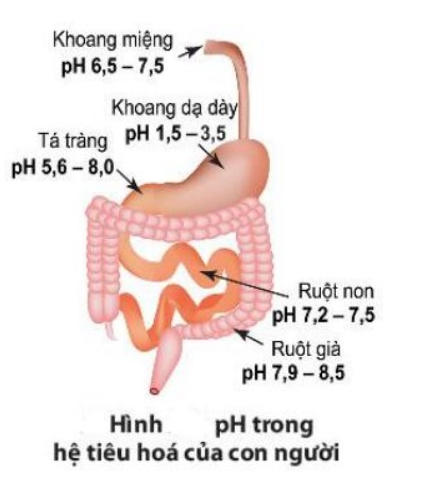
\includegraphics[width=6.5cm]{images_crop_hoa11_de02/cau15_ph_he_tieu_hoa.png}
\end{center}
\choice
{Dung dịch sodium hydrogen carbonate}
{Nước đun sôi để nguội}
{Nước đường saccarose}
{Một ít giấm ăn}
\loigiai{}
\end{ex}

\begin{ex}
Để trung hòa $20\text{ mL}$ dung dịch $\ce{HCl}\ 0{,}1\text{ M}$ cần $10\text{ mL}$ dung dịch $\ce{NaOH}$ nồng độ $x\text{ mol/L}$. Giá trị của $x$ là
\choice
{$0{,}3$}
{$0{,}4$}
{$0{,}2.$}
{$0{,}1.$}
\loigiai{}
\end{ex}

\begin{ex}
Trong dung dịch muối dichromate luôn có cân bằng:
\[\ce{Cr2O7^2- (da\ cam) + H2O <=> 2CrO4^2- (vang\ chanh) + 2H+}\]
Nếu thêm dung dịch acid $\ce{HBr}$ đặc và dư vào dung dịch $\ce{K2Cr2O7}$ thì dung dịch chuyển thành
\choice
{Màu da cam.}
{Màu vàng.}
{Màu xanh lục.}
{Không màu.}
\loigiai{}
\end{ex}

\begin{ex}
Cho các phát biểu sau:\\
(1) Phản ứng thuận nghịch là phản ứng xảy ra theo 2 chiều ngược nhau trong cùng điều kiện.\\
(2) Chất xúc tác có tác dụng làm tăng tốc độ phản ứng thuận và nghịch.\\
(3) Cân bằng hóa học là trạng thái mà phản ứng đã xảy ra hoàn toàn.\\
(4) Khi phản ứng thuận nghịch đạt trạng thái cân bằng hóa học, nồng độ các chất sẽ không đổi.\\
(5) Khi phản ứng thuận nghịch đạt trạng thái cân bằng hóa học, phản ứng dừng lại.\\
(6) Sự chuyển dịch cân bằng của phản ứng thuận nghịch $\ce{2NO2 <=> N2O4}$ không phụ thuộc sự thay đổi áp suất.\\
Số phát biểu sai là
\choice
{1.}
{2.}
{3.}
{4.}
\loigiai{}
\end{ex}

\Closesolutionfile{ans}

\bigskip
\noindent
\textbf{PHẦN II (4,0 điểm -- 4 câu): Câu trắc nghiệm đúng sai.}\\
\textit{Thí sinh trả lời từ câu 1 đến câu 4. Trong mỗi ý a), b), c), d) ở mỗi câu, thí sinh chọn đúng hoặc sai.}

\begin{ex}
Cho cân bằng hoá học trong bình kín: $\ce{2SO2(g) + O2(g) <=> 2SO3(g)}$, biết phản ứng thuận là phản ứng toả nhiệt.
\choiceTF
{Khi giảm nồng độ $\ce{O2}$, cân bằng chuyển dịch theo chiều nghịch.}
{Khi giảm nhiệt độ cân bằng chuyển dịch theo chiều thuận.}
{Khi giảm áp suất, cân bằng chuyển dịch theo chiều thuận.}
{Khi giảm nồng độ $\ce{SO3}$, cân bằng sẽ chuyển dịch theo chiều nghịch.}
\loigiai{}
\end{ex}

\begin{ex}
Cho các cân bằng sau:\\
(1) $\ce{2NH3(g) <=> N2(g) + 3H2(g)} \quad \Delta_r H^\circ_{298} > 0$\\
(2) $\ce{2SO2(g) + O2(g) <=> 2SO3(g)} \quad \Delta_r H^\circ_{298} < 0$\\
(3) $\ce{CaCO3(r) <=> CaO(r) + CO2(g)} \quad \Delta_r H^\circ_{298} > 0$\\
(4) $\ce{H2(g) + I2(g) <=> 2HI(g)} \quad \Delta_r H^\circ_{298} < 0$\\
Trong các cân bằng trên cân bằng nào sẽ chuyển dịch theo chiều thuận khi tăng nhiệt độ và giảm áp suất:
\choiceTF
{phương trình 1,2 sẽ chuyển dịch theo chiều thuận khi tăng nhiệt độ và giảm áp suất.}
{phương trình 1,3 sẽ chuyển dịch theo chiều thuận khi tăng nhiệt độ và giảm áp suất.}
{phương trình 1,2,3 cân bằng dịch theo chiều thuận khi giảm áp suất.}
{phương trình 4 cân bằng không chuyển dịch khi tăng áp suất.}
\loigiai{}
\end{ex}

\begin{ex}
Thực hiện thí nghiệm với 3 chất tan khác nhau là ethanol, potassium chloride và acetic acid như hình dưới đây:
\begin{center}
	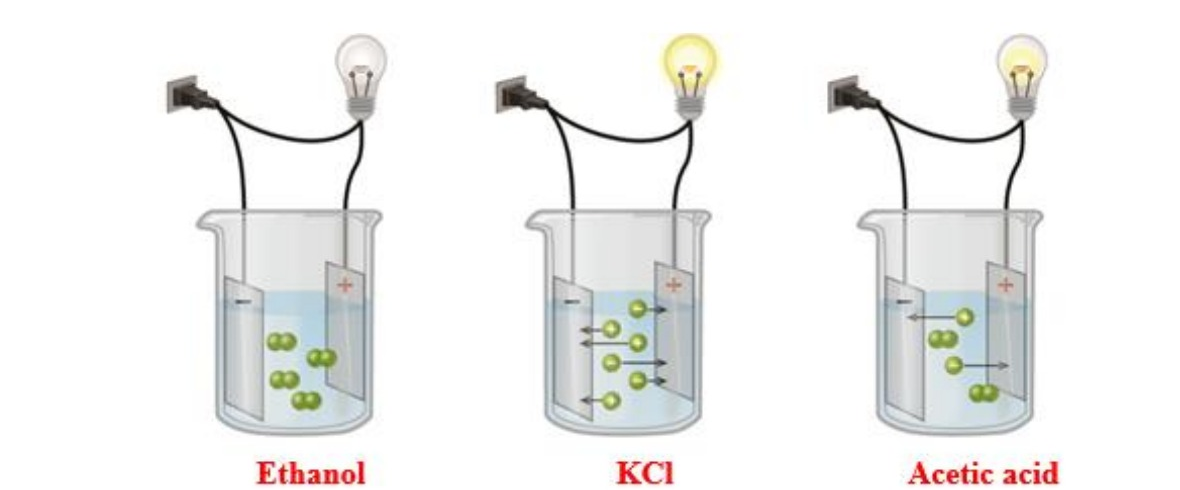
\includegraphics[width=11cm]{images_crop_hoa11_de02/cau3_p2_thi_nghiem_dan_dien.png}
\end{center}
\choiceTF
{Dung dịch $\ce{KCl}$ và acetic acid có khả năng dẫn điện.}
{Dung dịch hòa tan ethanol không dẫn điện.}
{Các phân tử acetic acid có 1 đầu mang điện dương và một đầu mang điện âm, chuyển động trong dung dịch tạo thành dòng điện.}
{Ethanol là chất điện li.}
\loigiai{}
\end{ex}

\begin{ex}
Trong lịch sử các thuyết về định nghĩa acid -- base có thuyết Arrhenius và thuyết Brønsted--Lowry:\\
-- Thuyết Arrhenius: ``Acid là chất phân ly trong dung dịch nước tạo thành $\ce{H+}$ (proton) còn base là chất phân ly trong dung dịch nước tạo thành $\ce{OH-}$''\\
-- Thuyết Brønsted--Lowry: ``Acid là chất cho proton ($\ce{H+}$) và base là chất nhận proton''
\choiceTF
{Theo thuyết Brønsted--Lowry phản ứng $\ce{HClO4 + CH3COOH <=> ClO4- + CH3COOH2+}$, trong phản ứng thuận thì $\ce{CH3COOH}$ là base, trong phản ứng nghịch thì $\ce{ClO4-}$ là acid.}
{Thuyết Brønsted--Lowry tổng quát hơn thuyết Arrhenius, vì phân tử không có nhóm --OH như $\ce{NH3}$, $\ce{SO3^2-}$, $\ce{CO3^2-}$ cũng là base.}
{Theo thuyết Brønsted--Lowry, các ion $\ce{Fe^3+}$, $\ce{Cu^2+}$, $\ce{Mg^2+}$, $\ce{Na+}$ được xem là acid.}
{Theo thuyết Arrhenius thì acid trong phân tử phải có nguyên tử H và base trong phân tử phải có nhóm --OH. Thuyết lí luận này đúng trong trường hợp dung môi sử dụng là nước.}
\loigiai{}
\end{ex}

\bigskip
\noindent
\textbf{PHẦN III (1,5 điểm -- 6 câu): Câu trắc nghiệm yêu cầu trả lời ngắn.}\\
\textit{Thí sinh trả lời từ câu 1 đến câu 6.}

\begin{ex}
Cho dãy các chất: $\ce{KAl(SO4)2.12H2O}$, $\ce{C2H5OH}$, $\ce{C12H22O11}$ (saccharose), $\ce{CH3COOH}$, $\ce{Ca(OH)2}$, $\ce{CH3COONH4}$. Số chất điện li là

\vspace{1.2cm}

\end{ex}

\begin{ex}
Cho các phản ứng:\\
(1) $\ce{NaOH + HCl -> NaCl + H2O}$\\
(2) $\ce{H2 + I2 <=> 2HI}$\\
(3) $\ce{CaCO3 <=> CaO + CO2}$\\
(4) $\ce{2KClO3 -> 2KCl + 3O2}$\\
Số phản ứng thuận nghịch là:

\vspace{1.2cm}

\end{ex}

\begin{ex}
\textbf{(SBT - CTST)} Trộn lẫn $V\text{ mL}$ dung dịch $\ce{NaOH}\ 0{,}01\text{ M}$ với $V\text{ mL}$ dung dịch $\ce{HCl}\ 0{,}03\text{ M}$ thu được $2V\text{ mL}$ dung dịch Y. Tính pH của dung dịch Y.

\vspace{1.2cm}

\end{ex}

\begin{ex}
Tính pH của dung dịch thu được sau khi trộn $40\text{ mL}$ dung dịch $\ce{HCl}\ 0{,}5\text{ M}$ với $60\text{ mL}$ dung dịch $\ce{NaOH}\ 0{,}5\text{ M}$.

\vspace{1.2cm}

\end{ex}

\begin{ex}
\textbf{(SBT - KNTT)} Ascorbic acid (vitamin C) là một acid hữu cơ được kí hiệu đơn giản là $\ce{HAsc}$, phân tử khối là 176. Một học sinh hoà tan $5{,}0\text{ g}$ ascorbic acid vào $250\text{ mL}$ nước. Tính pH của dung dịch thu được, biết trong dung dịch có cân bằng sau: $\ce{HAsc <=> H+ + Asc-}; K_a = 8 \cdot 10^{-5}$.

\vspace{1.2cm}

\end{ex}

\begin{ex}
\textbf{(SBT - KNTT)} Ethanol và propanoic acid phản ứng với nhau tạo thành ethyl propanoate theo phản ứng hoá học sau:
\[\ce{C2H5OH(l) + C2H5COOH(l) <=> C2H5COOC2H5(l) + H2O(l)}\]
Ở $50^\circ\text{C}$, giá trị $K_C$ của phản ứng trên là $7{,}5$. Nếu cho $23{,}0\text{ g}$ ethanol phản ứng với $37{,}0\text{ g}$ propanoic acid ở $50^\circ\text{C}$ thì khối lượng của ethyl propanoate thu được trong hỗn hợp ở trạng thái cân bằng là bao nhiêu gam? (Làm tròn đến hàng phần trăm).

\vspace{1.2cm}

\end{ex}

\bigskip
\noindent
\textbf{PHẦN IV: Tự luận}\\
\textit{Học sinh giải chi tiết các câu hỏi sau vào giấy làm bài.}

\begin{ex}
\textbf{[CD - SBT]} Quan sát Hình 1.1 và ghép mỗi đối tượng ở cột A với một mô tả thích hợp ở cột B:
\begin{itemize}
	\item \textbf{Cột A:} a) Đường (a); \quad b) $t_1$; \quad c) Đường (b); \quad d) $t_2$.
	\item \textbf{Cột B:} 1. không phải là thời điểm bắt đầu trạng thái cân bằng; \quad 2. mô tả biến thiên nồng độ chất sản phẩm theo thời gian; \quad 3. Là thời điểm phản ứng đạt trạng thái cân bằng; \quad 4. Mô tả biến thiên nồng độ chất phản ứng theo thời gian.
\end{itemize}
\begin{center}
	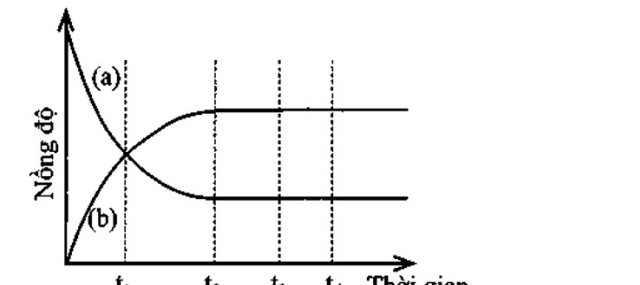
\includegraphics[width=7.5cm]{images_crop_hoa11_de02/cau1_p4_do_thi_nong_do.png}
\end{center}

\vspace{2.5cm}

\end{ex}

\begin{ex}
\textbf{[CD - SGK]} Trong môi trường acid, diệp lục có màu vàng đến đỏ; còn trong môi trường kiềm, diệp lục có màu xanh.\\
a) Giải thích vì sao khi vắt chanh vào nước luộc rau muống thì màu xanh của nước lại bị nhạt đi.\\
b*) Vì sao khi luộc bánh chưng, cho thêm một chút thuốc muối ($\ce{NaHCO3}$) sẽ làm lá dong gói bánh có màu xanh đẹp hơn?
\begin{center}
	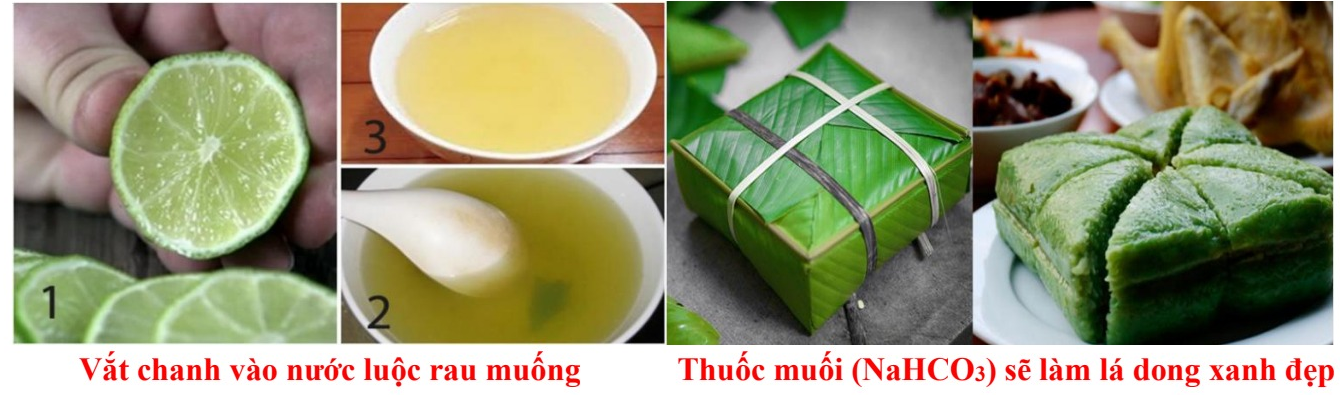
\includegraphics[width=10.5cm]{images_crop_hoa11_de02/cau2_p4_chanh_rau_muong_banh_chung.png}
\end{center}

\vspace{3.5cm}

\end{ex}

\begin{center}
\textbf{--------- HẾT ---------}
\end{center}

\end{document}
